\interlude[1]{Secure Channels}

\begin{frame}{Secure Channel Protocols}
  \begin{columns}[T]
    \begin{column}{.4\linewidth}
      \small

      Secure channel protocols like TLS, OpenSSH, or the Noise Protocol Framework \citeNoise  are used everywhere on the internet. They are

      \begin{itemize}
        \item Cheap
        \item Fast
        \item Secure
        \item Well analyzed
        \item Authenticated
        \item Usually not secure against quantum attacks
      \end{itemize}
    \end{column}
    \begin{column}{.55\linewidth}
     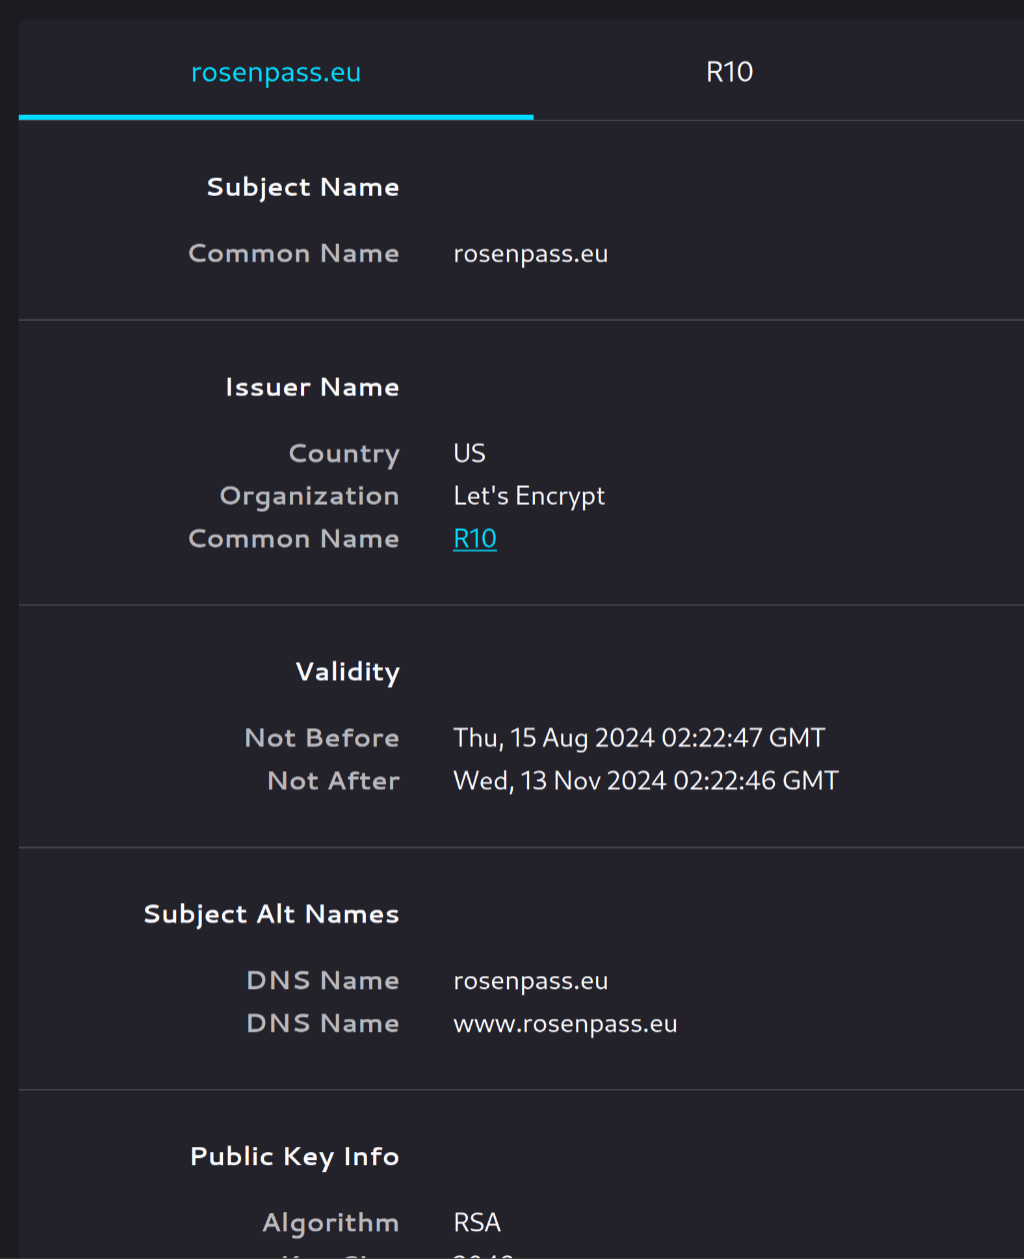
\includegraphics[width=\linewidth]{graphics/2024-09-13-rosenpass-tls-cert.png}
    \end{column}
  \end{columns}
\end{frame}

\begin{frame}{Security against quantum attacks}
  \begin{columns}[fullwidth,c]
    \begin{column}{.6\linewidth}
      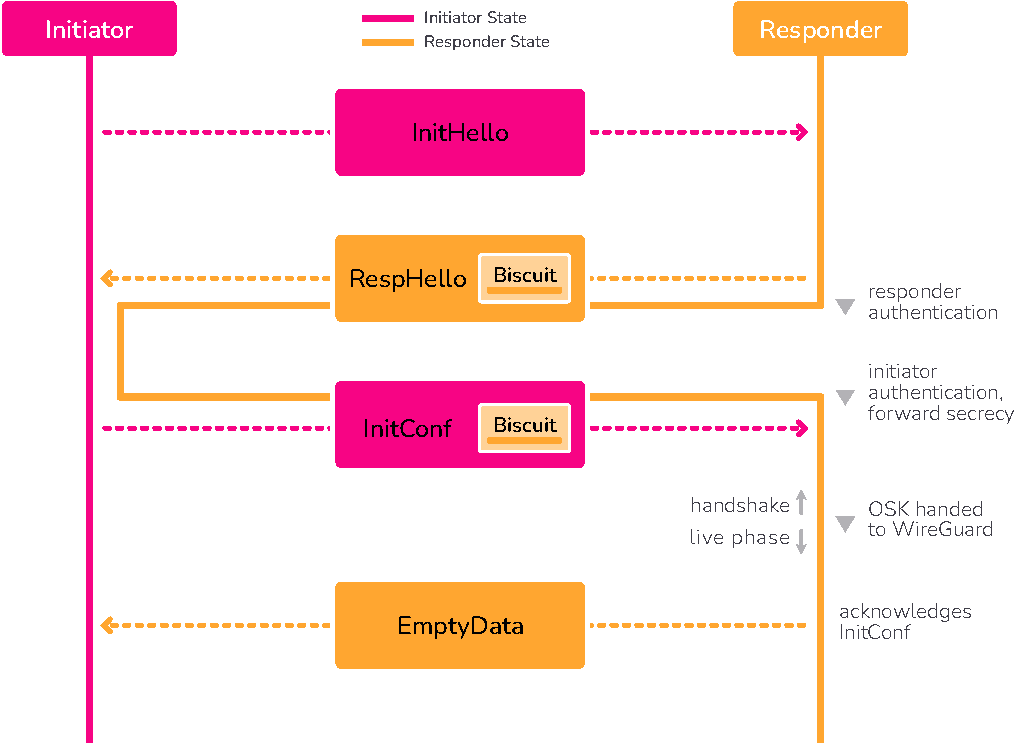
\includegraphics[height=\defaultframetextheight]{graphics/rosenpass-wp-key-exchange-protocol-rgb.pdf}
    \end{column}

    \begin{column}{.4\linewidth}
    \stretchcolumn{
    \vfill
      \begin{itemize}
        \item Migration to post-quantum security is definetly possible
        \item Rosenpass (pictured) is an example
        \item Alternatives such as KEM-TLS have also been proposed
        \item Some high security protocols such as OpenSSH and the Signal protocol are already using hybrid PQC
        \item Modest increase in resource usage
      \end{itemize}
      \vfill
      }
    \end{column}
  \end{columns}
\end{frame}

\interlude[1]{Secure channels: Security Properties}

\begin{frame}{Active \& Passive Security: Passive attacker}
  \includegraphics[width=.95\linewidth]{graphics-repo/comic/rosenpass-comic_03-interception1.jpeg}
\end{frame}

\begin{frame}{Active \& Passive Security: Active attacker}
  \raggedright
  \includegraphics[width=.95\linewidth]{graphics-repo/comic/rosenpass-comic_03-interception2.jpeg}
\end{frame}

\begin{frame}{Secrecy}
  \centering
  \includegraphics[width=.32\textwidth]{graphics-repo/comic/rosenpass-comic_04-secrecy1.jpeg}
  \includegraphics[width=.32\textwidth]{graphics-repo/comic/rosenpass-comic_04-secrecy2.jpeg}
  \includegraphics[width=.32\textwidth]{graphics-repo/comic/rosenpass-comic_04-secrecy3.jpeg}
\end{frame}

\begin{frame}{Authenticity}
  \centering
  \includegraphics[width=.32\textwidth]{graphics-repo/comic/rosenpass-comic_05-authenticity1.jpeg}
  \includegraphics[width=.32\textwidth]{graphics-repo/comic/rosenpass-comic_05-authenticity2.jpeg}
  \includegraphics[width=.32\textwidth]{graphics-repo/comic/rosenpass-comic_05-authenticity3.jpeg}
\end{frame}

\begin{frame}{Identity hiding}
  \centering
  \includegraphics[width=.32\textwidth]{graphics-repo/comic/rosenpass-comic_06-identity-hiding1.jpeg}
  \includegraphics[width=.32\textwidth]{graphics-repo/comic/rosenpass-comic_06-identity-hiding2.jpeg}
  \includegraphics[width=.32\textwidth]{graphics-repo/comic/rosenpass-comic_06-identity-hiding3.jpeg}
\end{frame}

\begin{frame}{Deniability}
  \centering
  \includegraphics[width=.32\textwidth]{graphics-repo/comic/rosenpass-comic_07-deniability1.jpeg}
  \includegraphics[width=.32\textwidth]{graphics-repo/comic/rosenpass-comic_07-deniability2.jpeg}
\end{frame}

\begin{frame}{Non-Repudiation}
  \centering
  \includegraphics[width=.32\textwidth]{graphics-repo/comic/rosenpass-comic_08-non-repudiation1.jpeg}
  \includegraphics[width=.32\textwidth]{graphics-repo/comic/rosenpass-comic_08-non-repudiation2.jpeg}
\end{frame}

\begin{frame}{Advanced properties}
  Often provided by secure messaging protocols such as Signal or MLS

  \begin{itemize}
    \item Post-compromise security (recovering security after a compromise)
    \item Group messaging
    \item Metadata obfuscation
    \item Asynchronous handshakes (one party offline)
  \end{itemize}
\end{frame}

\begin{frame}{Forward secrecy}
  TODO
\end{frame}

\begin{frame}{Everlasting secrecy}
  TODO
\end{frame}

\begin{frame}{QKD Caveats}
\def\Check{\cellcolor{rosenpass-lightblue}\Checkmark}
\def\Cross{\cellcolor{red!10}\XSolidBrush}
\def\Impractical{\cellcolor{yellow!20}{Impractical}}%TODO Ideas for some icon?
  \begin{columns}[fullwidth]
      % TODO(marei):
      % Can we use a light-green background for green, a light-red one for cross and a yellow one for impractical?
      % Can we generally make this look nice and graphic-y?
      \begin{tabular}{l c c}
        \textbf{Security property} & \textbf{QKD} & \multicolumn{1}{p{\widthof{\bfseries encryption}}}{\centering\bfseries Software encryption} \\

        Post-Quantum        & \Check           & \Check           \\
        Forward-secrecy     &                 & \Check           \\
        Everlasting-Secrecy & \Impractical     & \Cross           \\
        End-2-End           & \Impractical     & \Check           \\
        Active Attackers    & \Cross           & \Check           \\
        Authenticity        & \Cross           & \Check           \\
        Deniability         & \Cross           & \Check           \\
        Non-repudiation     & \Cross           & \Check           \\
        Identity hiding     & \Cross           & \Check           \\
      \end{tabular}\qquad
    \begin{column}{.48\textwidth}

      QKD is…

      \begin{itemize}
        \item Expensive
        \item Inefficient
        \item Everlasting secrecy would be nice, but is impractical for real-world setups
        \item Multi-hop security is impractical
        \item End-2-end security is missing entirely (no QKD on my end-user device fiesable for now)
      \end{itemize}
    \end{column}
    \hfill
  \end{columns}
\end{frame}
